

\documentclass{article}
\usepackage[utf8]{inputenc}
\usepackage{authblk}
\usepackage{setspace}
\usepackage[margin=1.25in]{geometry}
\usepackage{graphicx}
\graphicspath{ {./figures/} }
\usepackage{subcaption}
\usepackage{amsmath}
\usepackage{lineno}
\usepackage{algorithm}
\usepackage[noend]{algpseudocode}
\usepackage{graphicx}
\usepackage{cleveref}
%\addbibresource{refs.bib}
\linenumbers

\title{Classical and Quantum Computing for Airline Scheduling Problem}
\author[1]{Changjin Lim}

\date{}

%%%%%% Spacing %%%%%%
% Use paragraph spacing of 1.5 or 2 (for double spacing, use command \doublespacing)
\onehalfspacing

\begin{document}

\maketitle

%%%%%% Abstract %%%%%%
\begin{abstract}
\end{abstract}

%%%%%% Main Text %%%%%%
\section{Classical algorithm process}

Common notation and terminology:
\begin{itemize}
    \item $G=(V, E)$ = ``complete graph'', strongly connected graph representing connections between all nodes $V'$ in demand graph.
    \item $G'=(V',E')$ = ``demand graph'', a directed multi-graph, i.e., it allows multiple edges between the same pair of nodes. This multiplicity represents the demand frequency on the corresponding segment.    
    \item $G'_j=(V'_j,E'_j)$ = subgraph of "demand graph" traversed by agent $j$
    \item $c(E'_j)$ = cost of arcs $E'_j$ of demand graph, that must be covered by agent $j$  (Does not include cost of virtual arcs).
    \item $P_j$ = Directed walk of agent $j$ in the complete graph $G$
    
    \item $c(P_j)$ = cost of path of agent $j$ in the complete graph (including the cost of virtual arcs.)
    \item $m$ = number of agents available to serve the demand
\end{itemize}

\begin{subequations} \label{eq:maep_0}
\begin{alignat}{2}
&\min_{{P_1}, \ldots, P_m} & \, \, \max_{j \in \{1,\ldots,m\}} & \, \, c(P_j)
\\
& &  & \text{s.t. } \, \, E' \subset  P_1 \cup \ldots \cup P_m 
\\
&&& \,\, \, \,  P_j=\{e_{i,j}\} \subseteq G \qquad \forall j=1\dots m
\end{alignat}
\end{subequations}
Objective
\begin{itemize}
    \item  Lower the maximum subgraph’s cost 
    \item Minimize the whole cost
\end{itemize}
Input
\begin{itemize}
    \item $G'$ 
    \item $m$
\end{itemize}
\subsection{Algorithm process}

%\begin{enumerate}
    %\item Graph partitioning algorithm    
    %\item Edge modification algorithm
    %\item TSP-Eulerian path finding algorithm
%\end{enumerate}

This algorithm can be divided in three parts. First, used partitioning algorithm for dividing the original graph. After partitioning, for lowering the maximum subgraph's cost applying edge modification algorithm. After Edge modification algorithm, Change the graph form to the TSP form. And it can make the result with solving TSP and finding Eulerian path. But before starts to explain the algorithms, we explain the Path finding algorithm first. Path finding algorithm is used in the subsequent algorithms for finding an Eulerian paths.
\subsection{Path finding algorithm}
The path finding algorithm is used in rest of the our algorithm. We find the Eulerian paths using greedy approach. The algorithm starts with arbitrary vertex, and check the arcs from the vertex to another vertex. Among the checked arcs, select the maximum cost arcs and proceed to that direction. We need both path that has limit and path that doesn't have limit. Because Edge modification algorithm needs path that has limit for balancing. But in TSP-Eulerian path finding algorithm needs all path regardless of limit. If path has limit, check the path and if the path over the limit then return the path. If path doesn't have limit, proceed until there has no arcs to proceed. After proceeding to forward, we need to search backward too. Back to the start vertex and proceed backward. After that, the path is returned.
\\
\\ Notation and Terminology:
\begin{itemize}
    \item $V$: Set of vertex
    \item $e_{u,v}$: Arc from $u$ to $v$
    \item $P$: The Eulerian path to return
\end{itemize}

\begin{algorithm}
    \caption{Path finding algorithm}
    \begin{algorithmic}[1]
        \Procedure {Pathfinding}{$V$,$\delta$}
        \State $P \leftarrow \emptyset$
        \State $u$ is selected randomly from $V$
        \State $P \leftarrow$ \Call{Forwardsearch}{$P,\delta,V,u$}
        \State $P \leftarrow$ \Call{Backwardsearch}{$P,\delta,V,v$}
        \State \Return P
        \EndProcedure
    \end{algorithmic}
\end{algorithm}

\begin{algorithm}
    \caption{Forwardsearch}
    \begin{algorithmic}[1]
        \Procedure {Forwardsearch}{$P$,$\delta,V,u$}
            \While{$c(P)<\delta$}
                \State $v$ $\leftarrow$ arg max$_{v \in V}$ $c(e_{u,v})$
                \State $P$ $\leftarrow$ $P \cup e_{u,v}$
                \State $u$ $\leftarrow$ $v$
            \EndWhile
            \State \Return $P$
        \EndProcedure
    \end{algorithmic}
\end{algorithm}

\begin{algorithm}
    \caption{Backwardsearch}
    \begin{algorithmic}[1]
        \Procedure {Backwardsearch}{$P$,$\delta,V,v$}
            \While{$c(P)<\delta$}
                \State $u$ $\leftarrow$ arg max$_{u \in V}$ $c(e_{u,v})$
                \State $P$ $\leftarrow$ $P \cup e_{u,v}$
                \State $v$ $\leftarrow$ $u$
            \EndWhile
            \State \Return $P$
        \EndProcedure
    \end{algorithmic}
\end{algorithm}

\subsection{Graph partitioning algorithm}
Graph partitioning algorithm is used for dividing the original graph to the multiple graphs. This process for using multi agents on the problem. In partitioning, one of the hueristic algorithm named NE(Neighbor Expansion)\cite{66d1ad1e8f1c43b88f191328697d8711} is used. NE makes the subgraphs’ cost balanced by partitioning with setting the upper limit of the cost that each subgraphs can have; So this algorithm is partitioned by repeating the process of dividing the original graph as much as the limit that the subgraph can have. The limit is usually set to the value that is original cost divided by the number of agents.
\\
\\ Notation and Terminology
\begin{itemize}
    \item $C$, $S$: Set of vertices
    \item $x$, $y$, $z$: Vertex
    \item $\delta$: The partitioned subgraphs' cost upper bound
    \item $E^{NE}_k$: Set of allocated edges in $k$th iteration
    \item $E^{NE}$: Set of edges in the graph
    \item $e_{u,v}$: The arc from vertex $u$ to vertex $v$
    \item $N(v)$: Set of vertices that is connected with vertex $v$
    \item exit: Flag for exiting iteration
    
    \item $V$: Set of all vertices in the graph
\end{itemize}
\begin{figure}
\centering
    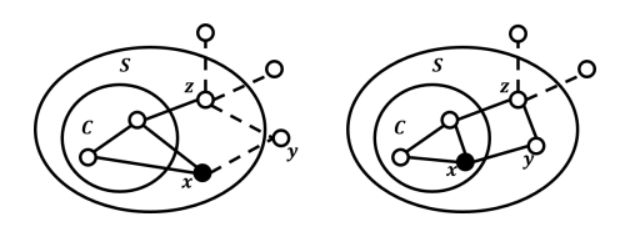
\includegraphics[width=\textwidth]{NE.png}
    \caption{Illustrating a step in the algorithm. Left: a vertex $x$ is selected. Right: the vertex set $C$, $S$, and the edge set $E^{NE}_k$ are updated. \cite{66d1ad1e8f1c43b88f191328697d8711}}
\end{figure}

The $C$, $S$, $x$, $y$, $z$ are used for explanation the Neighbor Expansion algorithm, so they are defined during the algorithm. The $\delta$ ,which is upper bound of each partitioned subgraphs' cost is used for balanced partitioning. It is the input parameter and it is obtained by dividing the total cost by the number of agents($c(G')/m$). In each iteration, arcs are allocated on $E^{NE}_k$. If it is bigger than $\delta$, the iteration is terminated. So, this algorithm is run for obtaining $m$ subgraphs. In last iteration, the remaining arcs $E^{NE}$ are finally partitioned and the algorithm is terminated.
\begin{algorithm}[H]
    \caption{Neighbor Expansion}
    \begin{algorithmic}[1]
        \Procedure {NE}{$E^{NE}$,$m$,$\delta$}
            \State exit $\leftarrow$ False
            \For{$k \in {1,2 ... m}$}
                \State $C,S,E^{NE}_k \leftarrow \emptyset$
                \While{$c(E^{NE}_k) \leq \delta $}
                    \If {$S\,\backslash\,C = \emptyset$}
                         \State $x$ is selected randomly in V $\backslash$ $C$
                    \Else 
                        \State $x \leftarrow$ $\underset{}{\operatorname{arg\,min_{v\in S \backslash C}}}$ $|N(v) \, \backslash \, S|$
                    \EndIf
                    \State $C \, \leftarrow \, C \cup \{x \}, S \, \leftarrow \, S \cup \{x \}$
                    \For{$y \in N(x) \, \backslash \, S$}
                        \State $S \, \leftarrow \, S \cup \{y\}$
                        \For{$z \in N(y) \cap S$}
                            \If{$e_{y,z} \in E^{NE}$}
                                \State $E^{NE}_k\, \leftarrow \, E^{NE}_k \cup \{e_{y,z}\}$
                                \State $E^{NE} \, \leftarrow \, E^{NE} \, \backslash \, \{e_{y,z}\}$
                            \EndIf
                            \If{$c(E^{NE}_k) > \delta $}:
                                \State exit $\leftarrow$ True
                                \State \textbf{break}
                            \EndIf
                            \If{$e_{z,y} \in E^{NE}$}
                                \State $E^{NE}_k\, \leftarrow \, E^{NE}_k \cup \{e_{z,y}\}$
                                \State $E^{NE} \, \leftarrow \, E^{NE} \, \backslash \, \{e_{z,y}\}$
                            \EndIf
                            \If{$c(E^{NE}_k) > \delta $}\:
                                \State exit $\leftarrow$ True
                                \State \textbf{break}
                            \EndIf
                        \EndFor
                        \If{exit $=$ True}
                            \State \textbf{break}
                        \EndIf
                    \EndFor
                \EndWhile
            \EndFor
            \State \Return $\forall E^{NE}_k, E^{NE}$
        \EndProcedure
    \end{algorithmic}
\end{algorithm}

According to the algorithm process, all $E^{NE}_k$ that is saved on each iteration and lastly saved $E^{NE}$ are finally returned and they are saved as the partitioned subgraphs.

\subsection{Edge Modification algorithm}
Edge modification algorithm makes the graph to the balanced graph. We divided the graph on the first stage with NE algorithm. Before applying the Edge modification algorithm, find the biggest subgraph and the smallest subgraph among the subgraphs that are partitioned by NE algorithm. After that, find the path to move and transfer it from the biggest subgraph to the smallest subgraph.

\\
\\ Notation and Terminology:
\begin{itemize}
    \item $\delta'$: cost lower bound of the path to be modified
    \item $\hat{G}_{max}=(\hat{V}_{max},\hat{E}_{max})$: The subgraph which has the biggest cost among the partitioned $G'_j$
    \item $\hat{G}_{min}=(\hat{V}_{min},\hat{E}_{min})$: The subgraph which has the smallest cost among the partitioned $G'_j$
    \item $P$: It is a path that makes the cost difference between the two graphs similarly when $H$ is given from $G'_{max}$ to $G'_{min}$
\end{itemize}

First, we need to find out some path to modify. So we apply the Path finding algorithm with limit. The path limit is calculated by 
\begin{equation}
    \delta' = c(\hat{G}_{max})-(c(\hat{G}_{max})+c(\hat{G}_{min}))/2
\end{equation}
This is because when $\hat{G}_{max}$ give a path to the $\hat{G}_{min}$ $\hat{G}_{max}$ and $\hat{G}_{min}$ need to be balanced. After the path finding, remove the path from $\hat{G}_{max}$ and add the path to $\hat{G}_{min}$. The algorithm is terminated.

\begin{algorithm}
    \caption{Edge Modification algorithm}
    \begin{algorithmic}[1]
    \Procedure{EdgeModification}{$\hat{V}_{max},\delta'$}
        \State $P \leftarrow$ \Call{Pathfinding}{$\hat{V}_{max},\delta'$}
        \State $\hat{E}_{max} \leftarrow \hat{E}_{max} \backslash P$
        \State $\hat{E}_{min} \leftarrow \hat{E}_{min} \cup P$
        \State \Return $\hat{G}_{max},\hat{G}_{min}$
    \EndProcedure
    \end{algorithmic}
    
\end{algorithm}

\subsection{TSP-Eulerian path finding algorithm}
TSP-Eulerian path finding algorithm is used for making the subgraphs to the Eulerian path. This algorithm add arcs to each subgraphs minimizing the adding cost. This algorithm's process is as follows. First, find all path in the subgraph using Path finding algorithm with no limit. Next, check the arc's cost that arc from each paths' end node to another paths' start node from the fully connected graph G. After that, shrink each paths to a node and make fully connected graph using checked arcs before. Lastly, solve the TSP with fully connected graph and return the result path. The result path is the Eulerian path because each paths is the Eulerian path. If we apply this process to all subgraphs, we could get an Eulerian paths about each subgraphs.
\\
\\ Notation and Terminology:
\begin{itemize}
    \item $G'_k=(V'_k,E'_k)$: The kth subgraph
    \item $G_{SG}=(V_{SG},E_{SG})$: The shrunk graph that is complete graph with shrinking nodes
    \item $P_i$: The ith path in $G'_k$
    \item $P'_i$: The vertex shrunk path $P_i$
    \item $P_{i,start}$: Path $P_i$'s start node
    \item $P_{i,end}$: Path $P_i$'s end node
    \item $n$: The number of path
\end{itemize}

\begin{algorithm}[H]
    \caption{TSP-Eulerian path finding algorithm}
    \begin{algorithmic}[1]
    
        \State $E_{SG} \leftarrow \emptyset$
        \State $n \leftarrow 0$
        \While{$|E'_k|>0$}
            \State $P_{n} \leftarrow$ \Call{Pathfinding}{$V'_k,\delta=\infty$} \Comment{Because there is no limit on the path, $\delta$ is infinite}
            \State $E'_k \leftarrow E'_k \backslash P_{n}$ 
            \State ${n} \leftarrow n+1$
        \EndWhile
        \For{$j \in {1...n}$}
            \For{$k \in {1...n}$}
                \If{$j \ne k$}
                    \State $E_{SG} \leftarrow E_{SG} \cup e(P'_j,P'_k)$
                    \State $c(e(P'_j,P'_k)) \leftarrow c(e(P_{j,start},P_{k,end}))$ \Comment{$c(e(P_{j,start},P_{k,end}))$ can be checked on G}
                \EndIf
            \EndFor
        \EndFor
        \State $Path \leftarrow$ \Call{TSP}{$G_{SG}$} \Comment{TSP can be solved by using B\&B algorithm}
        \State \Return $Path$
    \end{algorithmic}
\end{algorithm}


\subsubsection{Example for comprehension}
We will show you the toy example of TSP-Eulerian path finding algorithm for comprehension. The example graph has only 4 nodes and 2 arcs. we will show the process according to algorithm with picture.
\begin{enumerate}
    \item The example graph
    \begin{figure}[H]
        \centering
        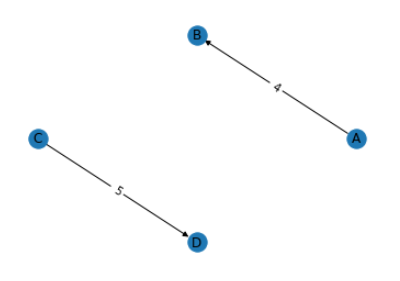
\includegraphics[width=10cm,height=7cm]{ex_img1.png}
        \caption{4 nodes, 2 arcs weighted directed graph}
    \end{figure}
    
    \newpage
    \item Check the graph's paths with Path finding algorithm
    \begin{figure}[H]
        \centering
        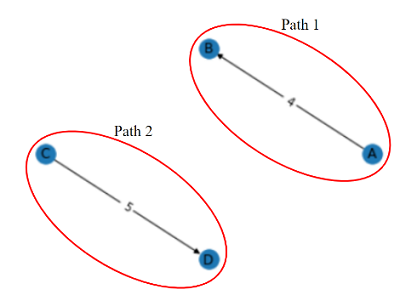
\includegraphics[width=10cm,height=7cm]{ex_img2.png}
        \caption{This graph has two Eulerian paths}
    \end{figure}

    \item Check the arcs cost that connects between paths.
    \begin{figure}[H]
        \centering
        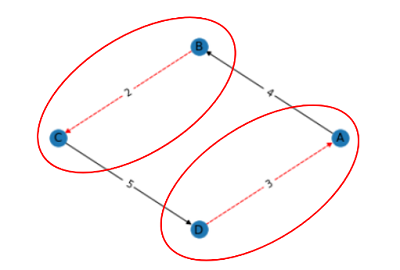
\includegraphics[width=10cm,height=7cm]{ex_img3.png}
        \caption{Check the two arcs cost}
    \end{figure}
    \newpage
    \item Shrink the paths to vertices
    \begin{figure}[H]
        \centering
        \begin{subfigure}{0.4\textwidth}
        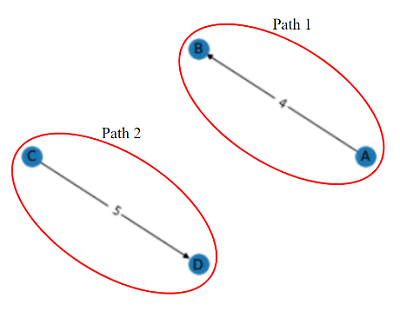
\includegraphics[width=\textwidth]{ex_img4.png}
        
        \end{subfigure}
        \hfill
        \begin{subfigure}{0.5\textwidth}
        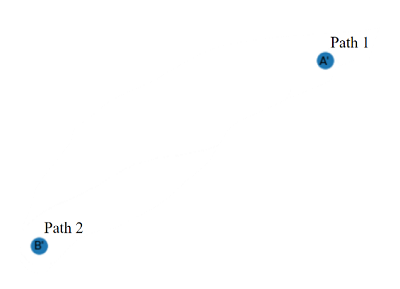
\includegraphics[width=\textwidth]{ex_img5.png}
        \end{subfigure}
        \caption{Paths shrunk to vertices}
    \end{figure}
    \item Make fully connected graph with the shrunk vertices and the checked arcs
    \begin{figure}[H]
        \centering
        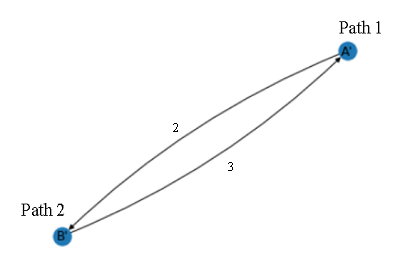
\includegraphics[width=10cm,height=7cm]{ex_img6.png}
        \caption{Input the two arcs cost}
    
    \end{figure}
    \newpage
    \item Solve TSP with the graph
    \begin{figure}[H]
        \centering
        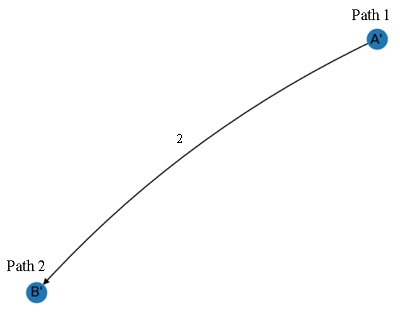
\includegraphics[width=10cm,height=7cm]{ex_img7.png}
        \caption{Result graph}
    \end{figure}
\end{enumerate}

After we solve TSP, we can get an Eulerian path about this graph.

\section{Results}


\section{Discussion}



%\printbibliography
{\small 
\bibliographystyle{unsrt}
\bibliography{./refs.bib}
}

\end{document}


